\documentclass{article}
\usepackage[utf8]{vietnam} %Gói dùng tiếng Việt%
\usepackage[left=3.5cm,right=2.5cm,top=2cm,bottom=2cm]{geometry}  %Gói canh lề%

\usepackage{minitoc} %Gói mục lục động %
\usepackage{xurl} 
\usepackage{scrextend}
%Begin: Giao diện mục lục
\usepackage{hyperref}
\hypersetup{
    colorlinks=true,
    linkcolor=blue,
    filecolor=magenta,      
    urlcolor=cyan,
    pdftitle={Overleaf Example},
    pdfpagemode=FullScreen,
    }
\urlstyle{same}
%End: Giao diện mục lục
\usepackage{subfigure}
%End: Thêm các package cần thiết%
\changefontsizes{14pt}
\setlength{\parindent}{0pt}
% %Begin: Thêm watermark%
% \usepackage{draftwatermark} %Gói watermark%
% \SetWatermarkAngle{45}
% \SetWatermarkColor[gray]{0.97}
% \SetWatermarkFontSize{5cm}
% \SetWatermarkText{KNNN EZI}
% %End: Thêm watermark%
\usepackage{graphicx}
\usepackage{amsmath}
\newcommand\tab[1][1cm]{\hspace*{#1}}
\title{Truonw Cong Nghe Thong Tin}
\author{duc viet}
\date{may 2022}
\begin{document}
\begin{titlepage}
    %Begin: Bìa%
    \begin{center}
        \vspace{5pt}
        \textbf{ĐẠI HỌC QUỐC GIA THÀNH PHỐ HỒ CHÍ MINH}
        \vspace{5pt}
        \textbf{TRƯỜNG ĐẠI HỌC CÔNG NGHỆ THÔNG TIN}
    \end{center}
    
    \vspace{5pt}
    
    \begin{center}
        
\includegraphics[scale=0.3]{BT/UIT}
        \vspace{10pt}
        \fontsize{15pt}{15pt}\selectfont
    
        \begin{flushleft}
        \fontsize{15pt}{15pt}\selectfont  
        \textbf{\textsl{MÔN HỌC:}~~~{PHÂN TÍCH VÀ THIẾT KẾ THUẬT TOÁN}}
        \end{flushleft}
    \end{center}
    
    
    \begin{flushleft}
        \fontsize{15pt}{15pt}\selectfont  
        \textbf{\textsl{ĐỀ TÀI:}~~~~~~~{BÀI TẬP NHÓM SỐ 1}}
    \end{flushleft}
    
    
    \vspace{15pt}
    \textbf{LỚP: CS112.O11}
    
    \vspace{10pt}
    \textbf{Nhóm sinh viên thực hiện:}
    \begin{tabbing}
    \hspace{9cm}\=\hspace{3cm}\=\ \kill
    {\it \textbf{Họ và tên}}\>{\it \textbf{MSSV}}\>\\
    \begin{bfseries}Nguyễn Hoàng Phúc\end{bfseries}\> \begin{bfseries}22521129\end{bfseries}\\
    \begin{bfseries}Đoàn Văn Hoàng\end{bfseries}\> \begin{bfseries}22520459\end{bfseries}\\
    \begin{bfseries}Nguyễn Viết Đức\end{bfseries}\> \begin{bfseries}22520273\end{bfseries}\\
    \end{tabbing}
    %End: Bìa%
    \vspace{10pt}
    \end{titlepage}
\newpage
\section*{Bài 1}

\vspace{5mm}
Câu a. 
\tab \(\text{S} = 1 + 3 + 5 + 7 +\dots + 999 = [\frac{999 - 1}{2} + 1]\frac{1+999}{2} = 250000\)

\vspace{5mm}
Câu b. 
\tab \(\text{S} = 2 + 4 + 8 + \dots + 1024 = \sum\limits_{i=1}^{10}{2^i} = \sum\limits_{i=0}^{10}{2^i} - 1 = 2046 \)

\vspace{5mm}
Câu c. 
\tab \(\sum\limits_{i=3}^{n+1}{1} = n+1-3+1 = n-1\)


\vspace{5mm}
Câu d. 
\tab \(\sum\limits_{i=3}^{n+1}{i} = \sum\limits_{i=1}^{n+1}{i} - \sum\limits_{i=1}^{2}{i} = \frac{(n+1)(n+2)}{2} - 3 = \frac{1}{2}x^2 + \frac{3}{2} - 2 \)

\vspace{5mm}
Câu e. 
\tab \(\sum\limits_{i=0}^{n-1}{i(i+1)} = \sum\limits_{i=0}^{n-1}{(i^2 + i)}\\
\tab \tab = \sum\limits_{i=0}^{n-1}{i^2} + \sum\limits_{i=0}^{n-1}{i} = \frac{1}{3}(n-1)^3 + \frac{1}{2}(n-1)^2
\)

\vspace{5mm}
Câu f. 
\tab \(\sum\limits_{j=3}^{n+1}{i} = \sum\limits_{i=1}^{n+1}{i} - \sum\limits_{i=1}^{2}{i} = \frac{(n+1)(n+2)}{2} - 3 = \frac{1}{2}x^2 + \frac{3}{2} - 2 \)

\vspace{5mm}
Câu i. 
\tab \(\sum\limits_{j\in (2,3,5)}^{ }{j^2 + j} \)

\section*{Bài 2}

- Xét vòng while ngoài:
Ta có:
\begin{itemize}
    \item $ 2+2n $(G)
    \item $ n + 1 $(SS)
\end{itemize}

Gọi $\alpha_{i}$ là số lần lặp lại vòng while trong.\\
Ta có: $\alpha_{i}$ là số con i chạy từ $ 1 -> i^2$, bước nhảy 1 \\
\(\Rightarrow \alpha_{i} = i^2 \)


\tab Suy ra:
\(
\begin{cases}
    \text{G(n) = } & 2 +2n +  \sum\limits_{i=1}^{n}2\alpha_{i} \\
    \text{SS(n) = } &  n + 1 + \sum\limits_{i=1}^{n}(\alpha_{i}+1)
\end{cases}
\)
\tab $\Leftrightarrow $
\(
\begin{cases}
    \text{G(n) = } & 2 +2n +  \frac{n(n+1)(2n+1)}{3} \\
    \text{SS(n) = } &  2n + 1 + \frac{n(n+1)(2n+1)}{6}
\end{cases}
\)
\section*{Bài 4}
% 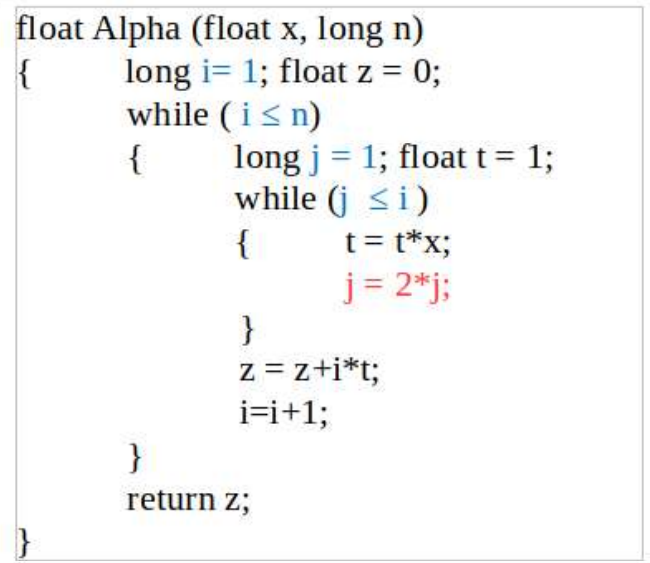
\includegraphics[scale=0.5]{BT/bai4}

- Xét vòng while ngoài:
Ta có:
\begin{itemize}
    \item $ 2+4*n $(G)
    \item $ n + 1 $(SS)
\end{itemize}

- Xét vòng while trong :
Đặt $\alpha_{i}$ là số vòng lặp của while trong, ta có:
\begin{itemize}
    \item $ 2*\alpha_{i}$ (G)
    \item $ \alpha_{i} + 1$ (SS)
\end{itemize}

\tab Suy ra:
\(
\begin{cases}
    \text{G(n) = } & 2 + 4n +  \sum\limits_{i=1}^{n}2\alpha_{i} \\
    \text{SS(n) = } &  n + 1 + n + \sum\limits_{i=1}^{n}\alpha_{i}
\end{cases}
\)
\vspace{5mm}

Xét $\alpha_{i}$ ta có:

\tab $\alpha_{i}$ là số con j với $j \leq  i$ , \(\text{Bước tăng theo tỉ lệ: } 2*j\)\\

\(\Rightarrow  \alpha_{i} \text{ là số phần tử của tập hợp } \{ 2^0, 2^1,  2^2, 2^3... \}
= k (\in 0 < 2^k \leq  i)\) 
\vspace{5mm}

\(\Leftrightarrow  1 \leq  2^k \leq  i\)

\vspace{2mm}
\(\Leftrightarrow  0 \leq k \leq  \log_{2}{i} \) 

\vspace{2mm}
\tab \(\Longrightarrow \alpha_{i} = \log_{2}{i} + 1\)\\


 Suy ra:
\(
\begin{cases}
    \text{G(n) = } & 2 + 4n +  \sum\limits_{i=1}^{n}2(\log_{2}{i} + 1) \\
    \text{SS(n) = } &  n + 1 + n + \sum\limits_{i=1}^{n}(\log_{2}{i} + 1)
\end{cases}
\)
 
\vspace{2mm}
\tab \(\Longleftrightarrow \)   
\(
\begin{cases}
    \text{G(n) = } & 2 + 6n +  \log_{2}{n!}  \\
    \text{SS(n) = } &  3n + 1 + \log_{2}{n!}
\end{cases}
\)


\section*{Bài 5}
% 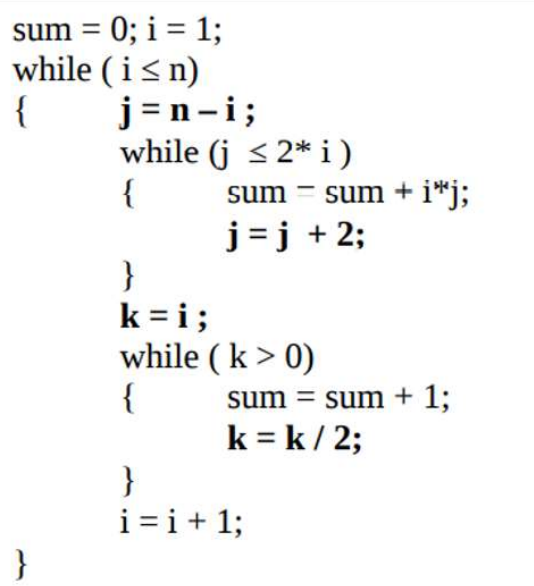
\includegraphics[scale=0.5]{BT/bai5}

- Xét vòng while ngoài:
Ta có:
\begin{itemize}
    \item $ 2 + 3*n $(G)
    \item $ n + 1 $(SS)
\end{itemize}

- Xét vòng $while_{(1)}$ trong :
Đặt $\alpha_{i}$ là số vòng lặp của while, ta có:
\begin{itemize}
    \item $ 2*\alpha_{i}$ (G)
    \item $ \alpha_{i} + 1$ (SS)
\end{itemize}

\vspace{15mm}

- Xét vòng $while_{(2)}$ trong :
Đặt $\beta_{i}$ là số vòng lặp của while, ta có:
\begin{itemize}
    \item $ 2*\beta_{i}$ (G)
    \item $ \beta_{i} + 1$ (SS)
\end{itemize}

\tab Suy ra:
\(
\begin{cases}
    \text{G(n) = } & 2 + 4n +  \sum\limits_{i=1}^{n}2\alpha_{i} + \sum\limits_{i=1}^{n}2\beta_{i} \\
    \text{SS(n) = } &  n + 1 + n + n + \sum\limits_{i=1}^{n}\alpha_{i} + \sum\limits_{i=1}^{n}\beta_{i}
\end{cases}
\)
\vspace{20mm}

Xét $\alpha_{i}$ ta có:

\tab $\alpha_{i}$ là số con j với $j \leq 2*i $ , \(\text{Bước tăng theo tỉ lệ: } 2\)\\

\(\Rightarrow  \alpha_{i} = \frac{3i - n}{2}\) 
\vspace{5mm}

Ta có:
\tab Vòng lặp $while_{(1)}$ trong chỉ thực hiện khi $ j \leq 2*i \Longleftrightarrow n/3 \leq i$

\vspace{5mm}
\(
\begin{cases}
    \alpha_{i} =  & \frac{3i-n}{2} \text{ , } i \geq n/3  \\
    \alpha_{i} =  & 0 \text{ , còn lại}
\end{cases}
\)
 
\vspace{20mm}
Xét $\beta_{i}$ ta có:

\tab $\beta_{i}$ là số con k với $k > 0 $ , \(\text{Bước giảm theo tỉ lệ: } 1/2\)\\


\(\Rightarrow  \beta_{i} \text{ là số phần tử của tập hợp } \{ \frac{i}{2^0}, \frac{i}{2^1},  \frac{i}{2^2},  \frac{i}{2^3}... \}
= k (\in 0 < \frac{i}{2^k} \leq i)\) 
\vspace{5mm}

\(\Leftrightarrow  1 \leq  \frac{i}{2^k} \leq  i\)

\vspace{2mm}
\(\Leftrightarrow  1 \leq  2^k \leq  i\)

\vspace{2mm}
\(\Leftrightarrow  0 \leq k \leq  \log_{2}{i} \) 

\(\Rightarrow  \beta_{i} = \log_{2}{i} + 1 \text{ (c/m tương tự câu 4)}\) 
\vspace{10mm}

\tab Suy ra:
\(
\begin{cases}
    \text{G(n) = } & 2 + 4n +  \sum\limits_{i=n/3}^{n}2\frac{3i-n}{2} + \sum\limits_{i=1}^{n}2(\log_{2}{i} + 1) \\
    \text{SS(n) = } &  n + 1 + n + n + \sum\limits_{i=n/3}^{n}\frac{3i-n}{2} + \sum\limits_{i=1}^{n}(\log_{2}{i} + 1)
\end{cases}
\)

\tab $\Leftrightarrow $
\(
\begin{cases}
    \text{G(n) = } & 2 + 6n -  3*(\frac{1}{2}n^2 + 1) + \log_{2}{n!} \\
    \text{SS(n) = } &  4n + 1  - (\frac{1}{2}n^2 + 1) + \log_{2}{n!} 
\end{cases}
\)

\newpage

\section*{Bài 7}
- Xét vòng while ngoài:
Ta có:
\begin{itemize}
    \item $ 2+2n $(G)
    \item $ n + 1 $(SS)
\end{itemize}

Gọi $\alpha_{i}$ là số lần lặp lại vòng while trong.\\
Ta có: $\alpha_{i}$ là số con i chạy từ $ 1 -> x$, bước tăng 1 \\
\(\Rightarrow \alpha_{i} = x = (n-i)(i-3n) \)

Gọi $\beta_{i}$ là số lần lệnh count = count - 2 được thực hiện \((i \geq 2y \Leftrightarrow i \geq 2i - 4n )\)\\
Xét bảng dấu:\\
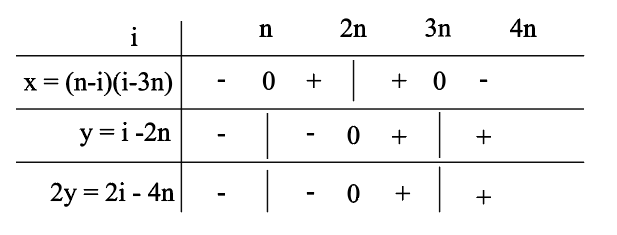
\includegraphics[scale=0.7]{BT/bangbai7}

\(\text{Lệnh } count = count - 2 \text{ được thực hiện khi } i \text{ chạy từ } 2n -> 3n -1\)

\tab $\Leftrightarrow \alpha_{i} = $
\(
\begin{cases}
    (n-i)(i-3n) & n < i < 3n \\
    0 & \text{, còn lại}
\end{cases}
\)
\vspace{10mm}

\tab \(\beta_{i} = 3n -1-2n+1 = n\)
\vspace{20mm}

\tab Ta có:
\(
\begin{cases}
    \text{G(n) = } & 2 + 16n +  \sum\limits_{i=1}^{4n}(\alpha_{i} + \beta_{i}) \\
    \text{SS(n) = } &  4n + 1  \sum\limits_{i=1}^{4n}(2\alpha_{i}+1)
\end{cases}
\)
\vspace{20mm}

\tab $\Leftrightarrow $
\(
\begin{cases}
    \text{G(n) = } & 2 + 16n +  \sum\limits_{i=n+1}^{3n-1}[(n-i(i-3n)) + n] \\
    \text{SS(n) = } &  8n + 3 + 2\sum\limits_{i=n+1}^{3n-1}[(n-i)(i-3n)]
\end{cases}
\)
\vspace{20mm}

\section*{Bài 8}
Gọi $\alpha_{i}$ là số lần lặp lại của vòng while trong,\\
\tab $\beta_{i-}$ là số lần lệnh $count = count - 1$ được thực hiện\\
\tab $ \beta_{i+}$ là số lần lệnh $count = count + 1$ được thực hiện\\
\tab $\gamma_{\acute{i}}$ là số lần $ y > 0$

\vspace{15mm}
\tab Suy ra::
\(
\begin{cases}
    \text{G(n) = } & 2 + 12n +  \sum\limits_{i=1}^{3n}(\alpha_{i} + \beta_{i-}) +  \beta_{i+}\\
    \text{SS(n) = } &  4n + 1  \sum\limits_{i=1}^{3n}(2\alpha_{i}+1) + \gamma_{\acute{i}}
\end{cases}
\)

\vspace{15mm}
Bảng xét dấu:\\
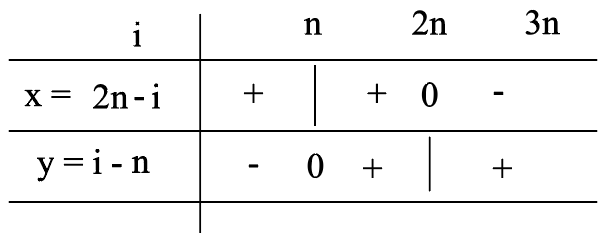
\includegraphics[scale=0.7]{BT/bangbai8}

\(=>\gamma_{\acute{i}} = 2n - (n+1) +1 = 2n \\
\tab \beta_{i+} =  2n - 1 - n + 1 = n \text{(vì khi y > 0 thì mới tiếp tục xét ) x > 0} \)

\vspace{10mm}
\tab $\alpha_{i} =$
\(
\begin{cases}
    2n - i & \text{, khi } 1 \leq i \leq 2n-1 \\
    0 & \text{, còn lại}
\end{cases}
\)

\vspace{10mm}
-Xét $\beta_{i-}$:\\
\tab \(n \leq j \leq x \Leftrightarrow n \leq j \leq 2n - i\\
\tab \text{.Nếu } 2n-i \geq n \Leftrightarrow  1 \leq i \leq n \text{ thì } \beta_{i-} \geq 1\)

\vspace{10mm}
\tab $\Rightarrow \beta_{i-} = $
\(
\begin{cases}
    n + 1 - i & \text{, khi } 1 \leq i \leq n \\
    0 & \text{, còn lại}
\end{cases}
\)

\vspace{20mm}
\tab Vậy:
\(
\begin{cases}
    \text{G(n) = } & 2 + 12n +  \sum\limits_{i=1}^{2n-1}(2n-i)  + \sum\limits_{i=1}^{n}(n+1-i) + n\\
    \text{SS(n) = } &  11n + 1 + 2\sum\limits_{i=1}^{2n-1}(2n-i)
\end{cases}
\)
\section*{Bài 9}
% 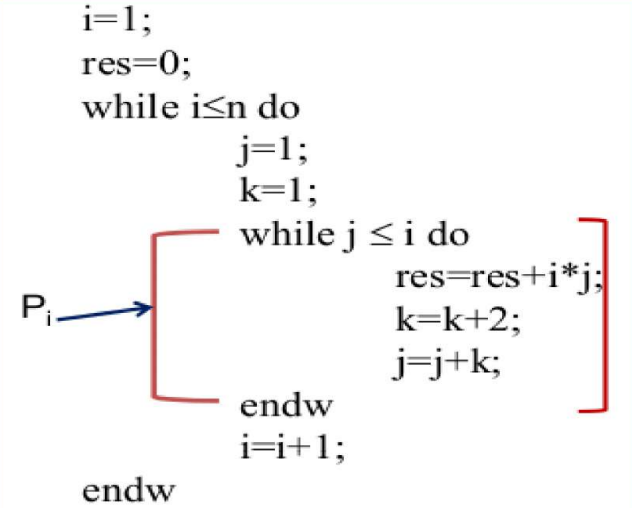
\includegraphics[scale=0.5]{BT/bai9}

- Xét vòng while ngoài:
Ta có:
\begin{itemize}
    \item $ 2 + 3*n $(G)
    \item $ n + 1 $(SS)
\end{itemize}

- Xét vòng while trong :
Đặt $\alpha_{i}$ là số vòng lặp của while, ta có:
\begin{itemize}
    \item $ 3*\alpha_{i}$ (G)
    \item $ \alpha_{i} + 1$ (SS)
\end{itemize}

\vspace{15mm}

\tab Suy ra:
\(
\begin{cases}
    \text{G(n) = } & 2 + 3n +  \sum\limits_{i=1}^{n}3\alpha_{i} \\
    \text{SS(n) = } &  n + 1 + n  + \sum\limits_{i=1}^{n}\alpha_{i} 
\end{cases}
\)

\vspace{15mm}
Xét $\alpha_{i}$ ta có:

\tab $\alpha_{i}$ là số con j với $j \leq i $ , \(\text{Bước tăng theo tỉ lệ: } j = j + k + 2\)\\

\(\Rightarrow  \alpha_{i} \text{ là số phần tử } \in \{ 1, 4, 9, 16, 25, ...\}\) 
\vspace{5mm}

Hay $ 1 \leq k^2 \leq i$
\vspace{5mm}

\(\Rightarrow  \alpha_{i} = \sqrt{i}\)


\vspace{5mm}
\tab Vậy:
\(
\begin{cases}
    \text{G(n) = } & 2 + 3n +  \sum\limits_{i=1}^{n}3\sqrt{i} \\
    \text{SS(n) = } &  n + 1 + n  + \sum\limits_{i=1}^{n}\sqrt{i} 
\end{cases}
\)

\vspace{5mm}
\tab  $\Leftrightarrow $
\(
\begin{cases}
    \text{G(n) = } & 2 + 3n +  \frac{3}{1/2 + 1}*n^{k+1} \\

    \text{SS(n) = } &  n + 1 + n  + \frac{1}{1/2 + 1}*n^{k+1} 
\end{cases}
\)
\end{document}
